\section{Discussion}
\label{sec:discussion}

ActiVCS allows to visualize a number of \glspl{kpi} and observe patterns in the project work. It also provides a tool that can be used for checking conformance to existing software development methodologies. 
\Cref{fig:zoom} shows a screenshot of the types of work Code and Test, taken from the \textsl{ok} project, described previously. A project manager can now check that work of the type Code and Test was consistently done throughout the lifetime of the project. Moreover, it is possible to observe that Code and Test were active together most of the time, with Code starting earlier. A typical development methodology that presents such pattern is \emph{agile}. 
\begin{figure}[]
    \centering
    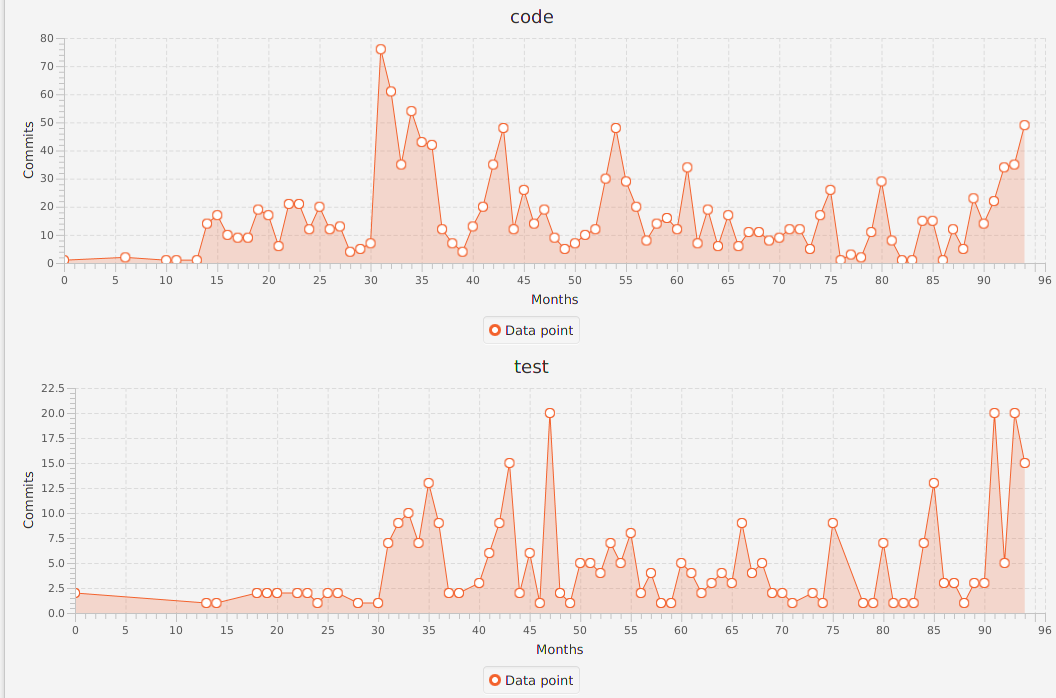
\includegraphics[width=\textwidth]{Project-mining-2-Mining-Type-of-Work/figures/ok-code-test}
    \caption{Zoom in on the evolution \textsl{Code} and \textsl{Test} activity types from the \textsl{ok} project}
    \label{fig:zoom}
\end{figure}


This might confirm that the \textsl{de facto} software development method corresponds with what the organization has decided. Alternatively, organization might be following a Waterfall development model. In that case, this pattern may point at a lack of control on the project. The managers can use their domain knowledge along with the provided \emph{factual} information for better decision making.

% Limitations of our technique are related to the preprocessing phase. The success of \gls{etl} procedure for obtaining the event log storage highly depends on properly formatting the \gls{vcs} log beforehand. As well, this step may be slow in case of large projects. 


